\documentclass{beamer}

\usetheme{Warsaw}
%\usecolortheme{lily} 
\setbeamercolor{frametitle}{bg=blue,fg=yellow} 
%\beamersetaveragebackground{blue!10} 

\newcommand{\supp}{\textrm{{s}upp}
}
\newcommand{\ce}{\mbox{\textnormal{{c}e}}
}
\newcommand{\card}{\mbox{\textnormal{{c}ard}}
}
\newcommand{\rc}{\mbox{\textnormal{rc}}
}
\newcommand{\sig}{\textrm{$\Sigma$Count}
}
\newcommand{\nf}{\mbox{\textnormal{nf$\sigma$-count}}
}
\newcommand{\req}[1]{(\ref{#1})}
\newcommand{\inn}{\mbox{\textnormal{in}}
}
\newcommand{\clm}{\mbox{\textnormal{clm}}
}

\usepackage[utf8]{inputenc}
\usepackage{amssymb}
\usepackage{graphicx} %for eps graphics
\usepackage[T1]{fontenc}
\usepackage[polish]{babel}
\usepackage{txfonts}
\usepackage{array}
\usepackage{graphicx}
\usepackage{caption}
\newcommand{\source}[1]{\caption*{Source: {#1}} }

\title{Kubernetes cluster deployment \\ for production environment}
%\toctitle{Kubernetes cluster deployment for production environment}

\author{Ewa Czechowska}
\institute{Lodz University of Technology}
\date{Łódź, 4th April 2020}

%\begin{frame}{\tableofcontents[currentsection]}
%\begin{frame}{\tableofcontents[currentsubsection]}

\begin{document}
\maketitle

\section{Introduction and definitions}
\subsection{Table of Contents}
\begin{frame}{Table of Contents}%{{{
\begin{center}
\begin{tabular}{@{}  l  l }
	\begin{figure}
		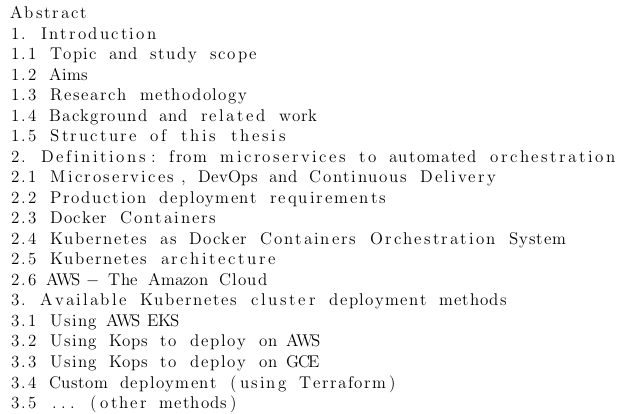
\includegraphics[width=5.5cm]{figures/table-of-c1.png}
		\label{fig:table-of-c1}
	\end{figure} &
	\begin{figure}
		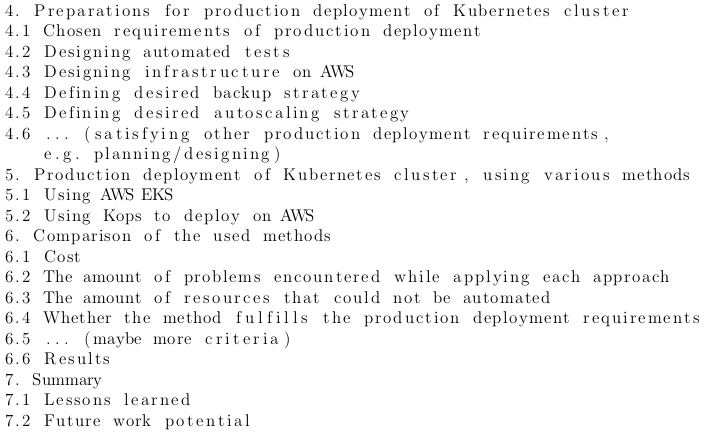
\includegraphics[width=5.5cm]{figures/table-of-c2.png}
		\label{fig:table-of-c2}
	\end{figure} \\
	\end{tabular}
\end{center}
\end{frame}
%}}}

\subsection{Topic and study scope}
\begin{frame}{Trends in IT}%{{{
\begin{itemize}
\item Architectural shift {\bfseries from monolith to microservices}
\item Migration {\bfseries from on-premises services to Cloud Native Applications}
\item Adoption of {\bfseries Docker containers}
\item Evolution of the movement: {\bfseries DevOps}
\end{itemize}
\end{frame}
%}}}

\begin{frame}{Docker containers - definition}%{{{
\begin{itemize}
\item Docker provides \textbf{a new way of virtualization}
\item Docker containers offer ready to use, installed, software packages including OS, software dependencies and runtime
\item Docker allows for quick deployments
\item \textbf{Virtual machines virtualize hardware, containers virtualize the operating system of a server}
\end{itemize}
\begin{figure}
	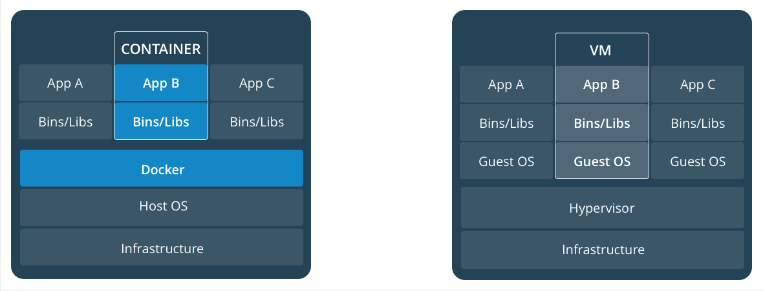
\includegraphics[width=6cm]{figures/docker-vs-vms.png}
	\label{fig:docker-vs-vms}
	\source{https://docs.docker.com/get-started/}
\end{figure}
\end{frame}
%}}}

\begin{frame}{Why follow trends?}%{{{
\begin{center}
	\begin{tabular}{ | c | c |}
		\hline
		{\bfseries Why microservices?} & {\bfseries Why Docker containers?} \\ \hline
		simpler architecture & portability across clouds \\ \hline
		reuse an application & limit "works on my machine" \\ \hline
		less context at once & faster startup times \\ \hline
		isolated failures &  light-weight \\ 
		\hline
	\end{tabular}
	\begin{tabular}{ | c |}
		\hline
		 {\bfseries Why cloud?} \\ \hline
		 scalability \\ \hline
		 lower upfront infrastructure investment \\ \hline
		 reliable hardware (SLAs) \\ \hline
		 efficient utilization of resources \\ 
		\hline
	\end{tabular}
\end{center}
\end{frame}
%}}}

%make the code architecture less coupled  & more efficient resources utilization & %Potential solutions\\ \hline
		% make the code architecture less coupled  & more efficient resources utilization & Potential solutions\\ \hline

% \begin{frame}{Why follow trends?}%{{{
% Why microservices?
% \begin{itemize}
% \item to simplify complex applications 
% \item to put less context into a developer's head
% \item to be able to easier navigate the failure

% Why migrate to cloud?
% \begin{itemize}
% \item to satisfy the need for scalability
% \item to decrease the upfront infrastructure investment
% \item to pay only for used infrastructure, not for the allocated part
% \item to utilize resources in a more efficient way
% \item to use reliable infrastructure (thanks to e.g. S3 SLA)
% \end{itemize}
% \end{frame}
% %}}}

% \begin{frame}{Why follow these trends?}%{{{
% Why choose Docker containers instead of virtual machines?
% \begin{itemize}
% \item to ensure such a deployment which is portable across infrastructure providers (across clouds)
% \item to avoid/decrease the frequency of the common problem "works on my machine"
% \item for faster startup times
% Docker instances are lighter-weight. To ship an app as a virtual machine image, you have to bake an entire operating system into the image. With a container, only the app itself has to go inside the container. This translates to a less complicated build process, plus the ability to host many more containers on a single physical server.
% \end{itemize}
% \end{frame}
% %}}}

\begin{frame}{Why Kubernetes? It is useful}%{{{
Challenges:
\begin{itemize}
	\item How to deploy a microservice if it depends on many other microservices?
	\item How to satisfy the need for scalability?
	\item How to ensure repetitive and fast deployments?
\end{itemize}

Solutions:
\begin{itemize}
	\item Use a containers' orchestrator like: Docker-compose, \textbf{Kubernetes}, Mesos, Docker Swarm
	\item Use \textbf{DevOps} practices like: Infrastructure as Code, Continuous Integration, Continuous Delivery, Configuration Management Systems
\end{itemize}
\end{frame}
%}}}

\begin{frame}{Kubernetes (k8s) - definition}%{{{
\begin{itemize}
\item An open-source system for \textbf{automating deployment, scaling, and management of containerized applications}
\item \textbf{Features}: self-healing, secret and configuration management, service discovery and load balancing, automated containers placing based on their resource requirements
\item Can be \textbf{deployed on many clouds} (AWS, GCP, Azure) or \textbf{on-premises} - unified experience
\item Bases \textbf{15 years of experience} of running production workloads at Google
\item A \textbf{CNCF} graduated project
\end{itemize}

\begin{tabular}{  c c }
	\begin{figure}
		
\includegraphics[width=3cm]{figures/kubernetes-logo.png}
		\label{fig:kubernetes-logo}
	\end{figure} &
	\begin{figure}
		
\includegraphics[width=3cm]{figures/cncf-logo.png}
		\label{fig:cncf-logo}
	\end{figure} 
\end{tabular}
\end{frame}
%}}}

\begin{frame}{Why Kubernetes? It is popular}%{{{
\begin{figure}
	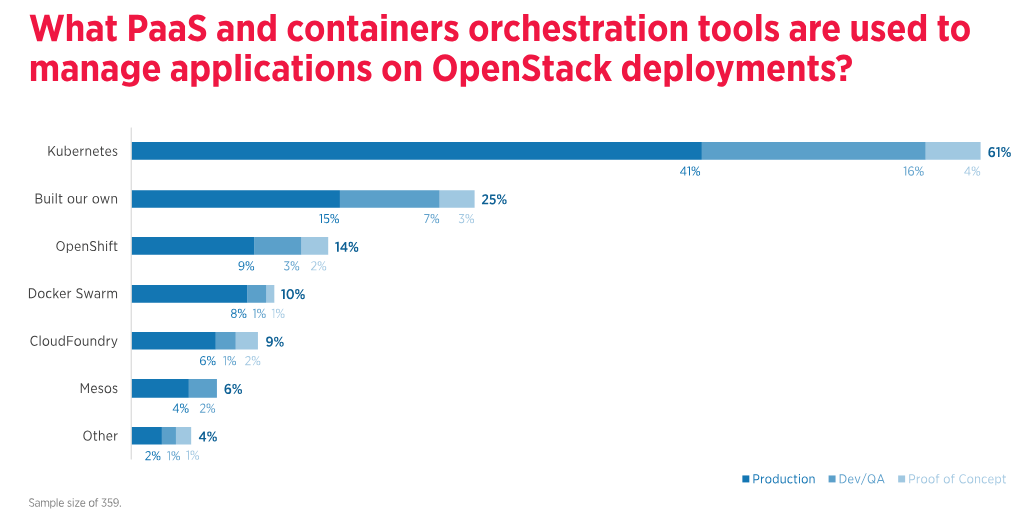
\includegraphics[width=10cm]{figures/k8s-openstack-survey.png}
	%\caption{Preferred containers orchestration tools on OpenStack, OpenStack Survey, 2018}
	\label{fig:k8s-openstack-survey}
	%\caption{Source: OpenStack Survey, 2018}
	\source{OpenStack Survey, 2018}
\end{figure}
\end{frame}
%}}}

\begin{frame}{Why Kubernetes? It is popular}%{{{
\begin{figure}
	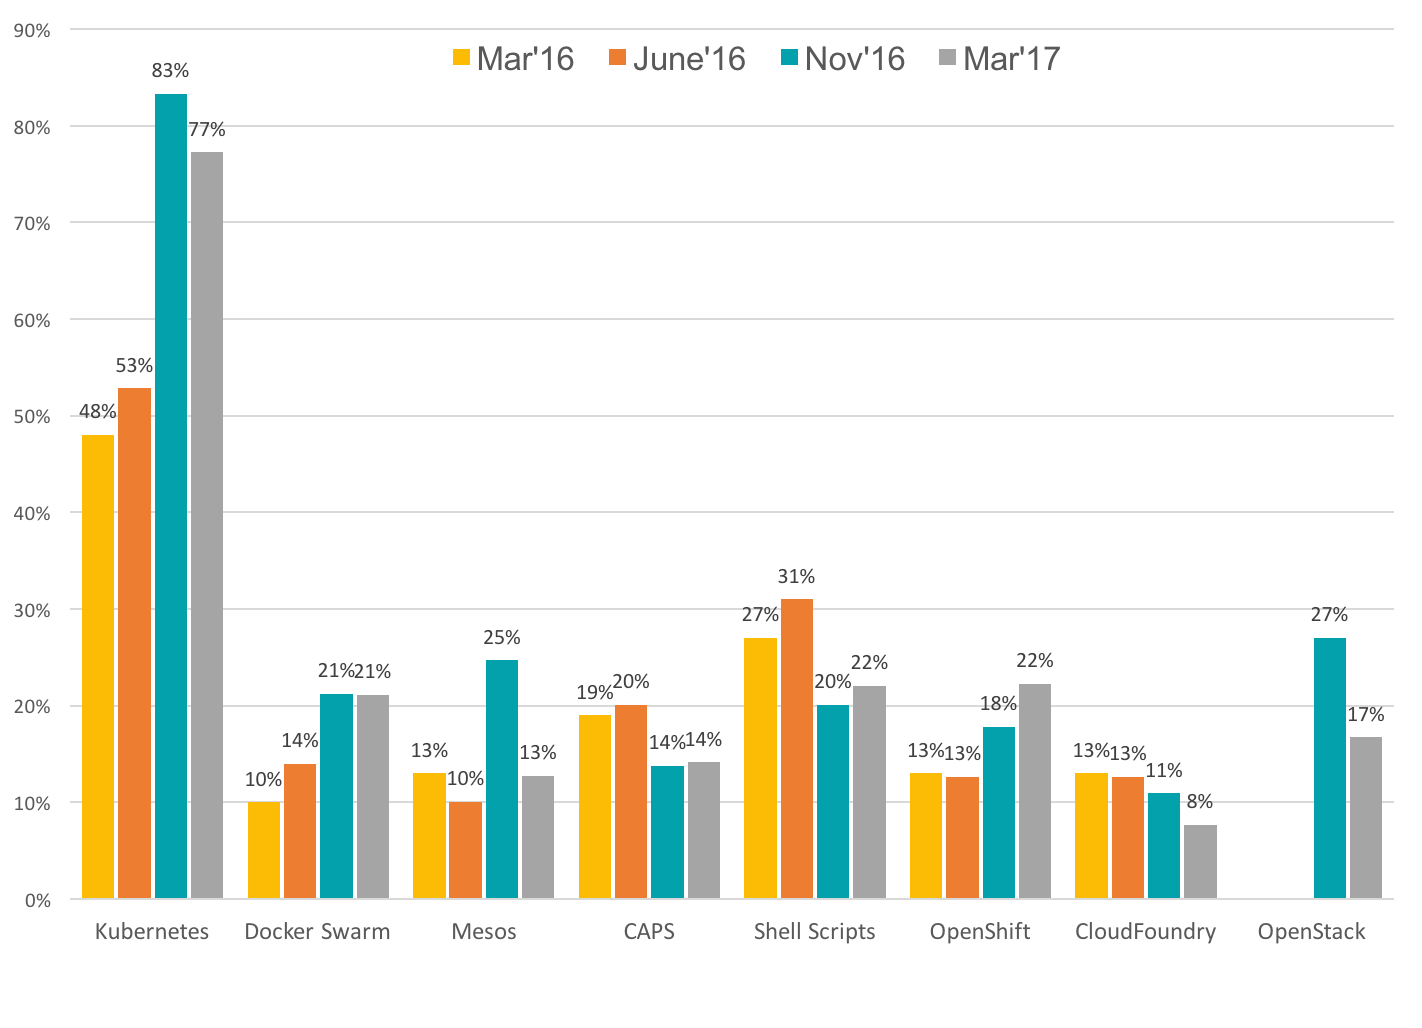
\includegraphics[width=8cm]{figures/cncf-container-orchestrators.png}
	%\caption{Preferred container management platforms, CNCF Survey, 2017}
	\label{fig:cncf-container-orchestrators}
	\source{CNCF Survey, 2017}
\end{figure}
\end{frame}
%}}}

\begin{frame}{Kubernetes is used in production environment}%{{{
\begin{figure}
	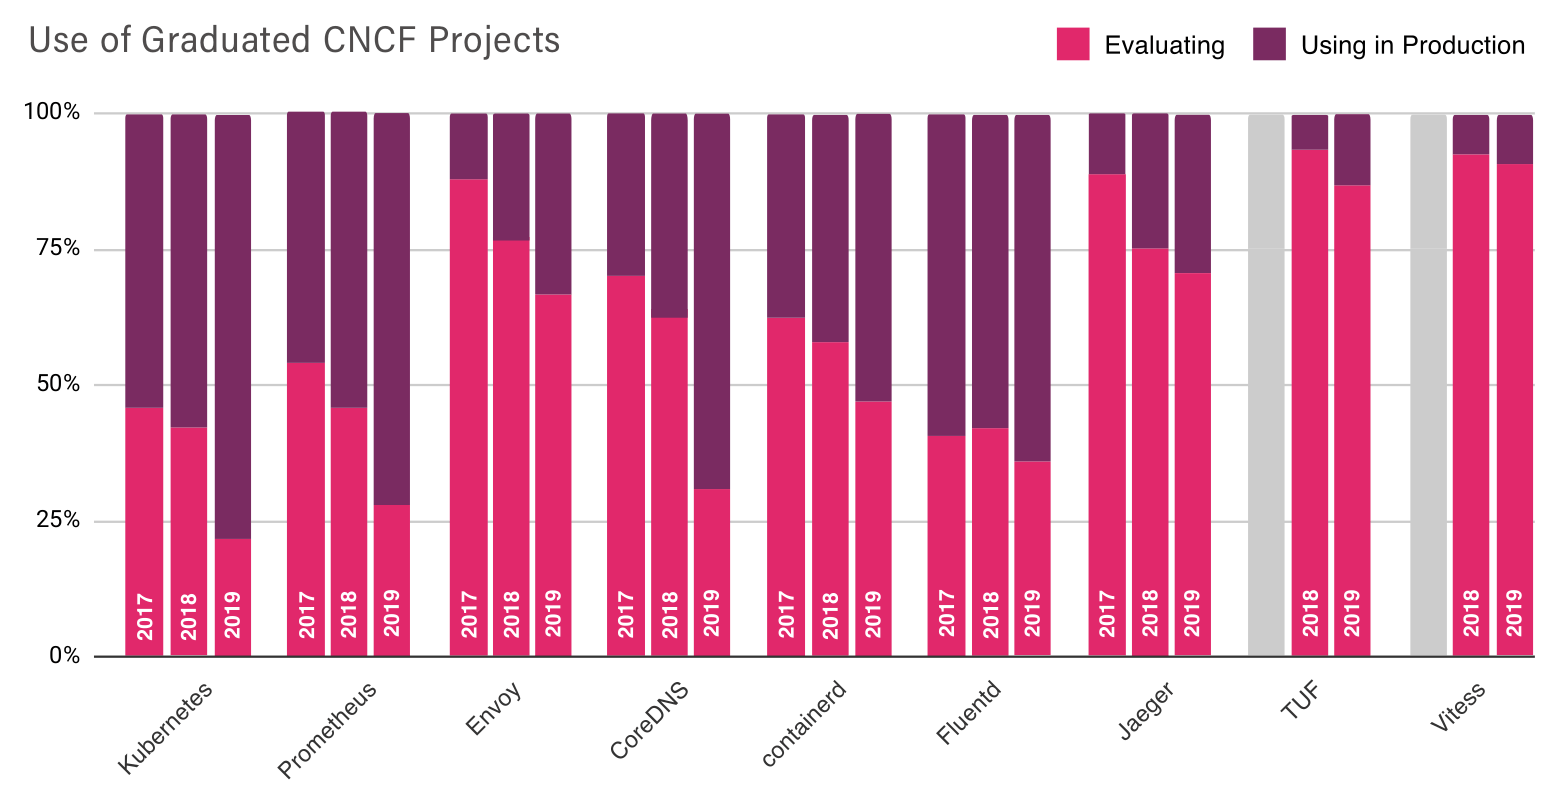
\includegraphics[width=10cm]{figures/cncf-k8s-used-in-production.png}
	\label{fig:cncf-k8s-used-in-production}
	\source{CNCF Survey, 2019}
\end{figure}
\end{frame}
%}}}

\begin{frame}{Kubernetes is used by NASA in production environment}%{{{
	\begin{figure}
		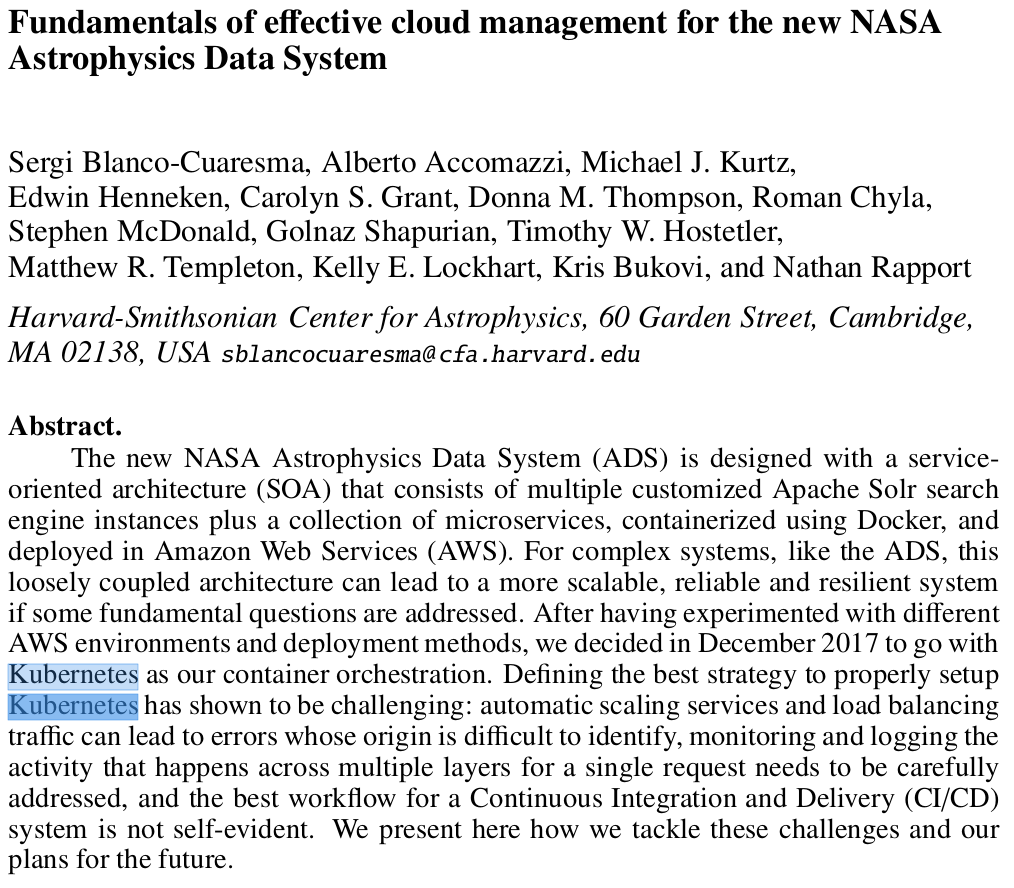
\includegraphics[width=6cm]{figures/k8s-used-by-nasa.png}
		\label{fig:k8s-used-by-nasa}
		\source{Fundamentals of effective cloud management for the new NASA Astrophysics Data System, 2019}
	\end{figure}
\end{frame}
%}}}

\begin{frame}{Methods how to deploy a Kubernetes cluster}%{{{
\begin{figure}
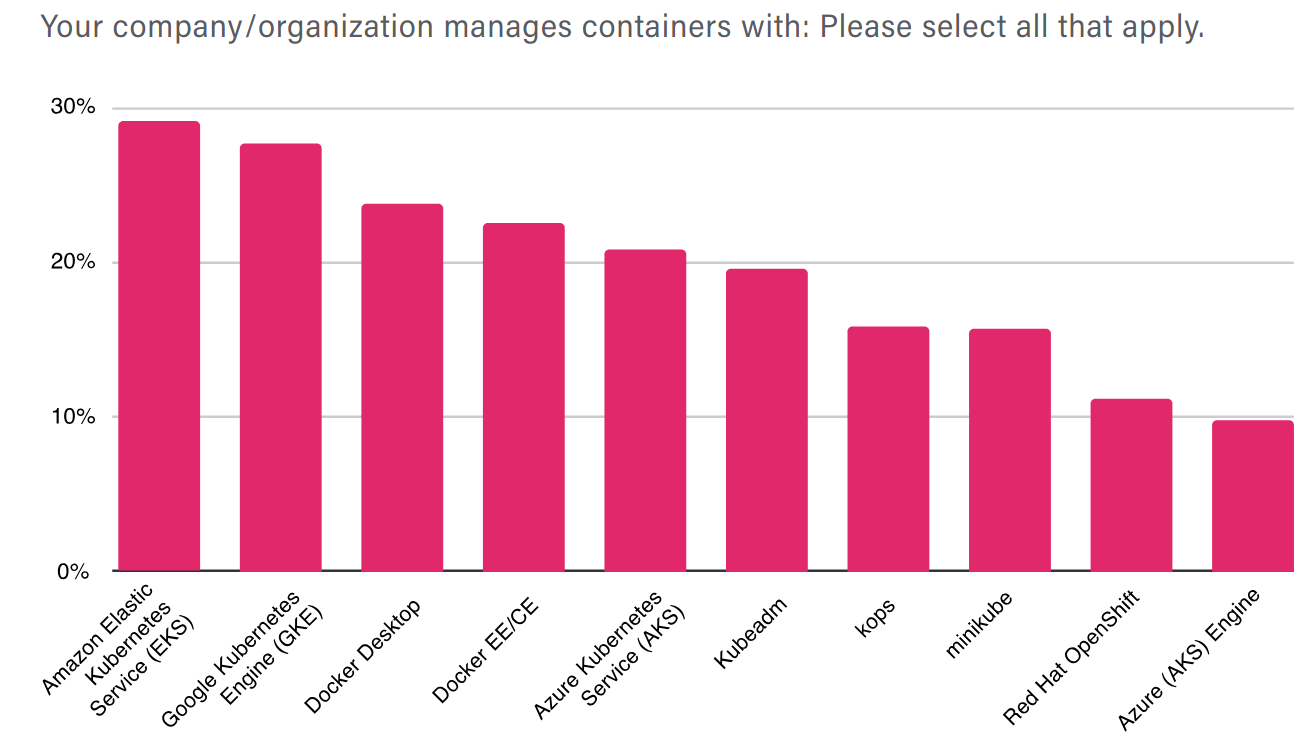
\includegraphics[width=8cm]{figures/cncf-k8s-deployment-methods.png}
\label{fig:cncf-k8s-deployment-methods}
\source{CNCF Survey, 2019}
\end{figure}
\end{frame}
%}}}

\begin{frame}{Why compare two deployment methods on AWS?}%{{{
	\begin{itemize}
		\item Kubernetes cluster deployment methods are described by blog posts and tutorials - not formal literature, but \textbf{practitioners use them}
		\item Comparison of two deployment methods on AWS is \textbf{not found in literature} (however usage of Kubernetes cluster in production environment was handled)
		\item \textbf{AWS is a stable cloud} with long history
		\item \textbf{AWS is popular} among practitioners
	\end{itemize}
\end{frame}
%}}}

\begin{frame}{Why focus on production environment?}%{{{
	\begin{itemize}
		\item To \textbf{facilitate others plan such deployment better} by letting them be aware upfront of its limitations and known issues
		\item To \textbf{apply a practical approach}
		\item To conform to the \textbf{DevOps best practices} and \textbf{Agile methodology}
	\end{itemize}
\end{frame}
%}}}

\subsection{About this study}
\begin{frame}{Aims and research methodology}%{{{
	\begin{itemize}
		\item Theoretical approach
		\begin{itemize}
			\item Search of existing literature (academic and other)
			\item Gather requirements of deployment in production environment
			\item Describe two deployment methods of Kubernetes cluster on AWS
		\end{itemize}
		\item Practical approach
		\begin{itemize}
			\item Perform the two deployments while conforming to the DevOps best practices and Agile methodology
			\item Compare these methods in the context of production environment
			\item List encountered problems and try to provide solutions
		\end{itemize}
	\end{itemize}
\end{frame}
%}}}

\begin{frame}{Related work - Formal literature}%{{{
\begin{itemize}
	\item Concern many clouds, practical approach, some production environment elements:
	\begin{itemize}
		\item \textbf{book}: Hideto, Saito, et. al. \textit{DevOps with Kubernetes}
		\item \textbf{book}: Sayfan, Gigi, et. al. \textit{Mastering Kubernetes}
	\end{itemize}
	\item \textbf{book}: Burns, Brendan, et. al. \textit{Kubernetes Up \& Running}. - many clouds, practical approach, no production environment elements
	\item \textbf{book}: Arundel, John, et. al. \textit{Cloud Native DevOps with Kubernetes}. - many clouds, theoretical approach
	\item \textbf{book}: Uphill, Thomas, et. al. \textit{DevOps: Puppet, Docker, and Kubernetes}. - AWS, practical approach
	\item \textbf{papers} acknowledge using Kubernetes, but do not explain details of its deployment
\end{itemize}
\end{frame}
%}}}

\begin{frame}{Related work - Informal literature}%{{{
\begin{itemize}
	\item \textbf{Many clouds compared, only theoretical approach}:
	\begin{itemize}
		\item https://platform9.com/blog/kubernetes-cloud-services-comparing-gke-eks-and-aks/
		\item https://logz.io/blog/kubernetes-as-a-service-gke-aks-eks/
		\item https://www.presslabs.com/blog/kubernetes-cloud-providers-2019/
	\end{itemize}
	\item \textbf{Practical approach, one method described}:
	\begin{itemize}
		\item https://eksctl.io/
		\item https://gruntwork.io/guides/kubernetes/how-to-deploy-production-grade-kubernetes-cluster-aws
		\item https://github.com/kelseyhightower/kubernetes-the-hard-way
		\item https://logz.io/blog/amazon-eks-cluster/
	\end{itemize}
\end{itemize}
\end{frame}
%}}}

\subsection{Production deployment requirements}
\begin{frame}{Production deployment requirements}%{{{
\begin{enumerate}
	\item Automation, Continuous Integration, Continuous Development, Infrastructure as Code
	\item Security
	\item High Availability, failover, fault-tolerancy
	\item Backup and restore, Disaster Recovery
	\item Centralized Monitoring
	\item Centralized Logging
	\item Centralized Audit
\end{enumerate}
\end{frame}
%}}}

\subsection{Kubernetes architecture}
\begin{frame}{Kubernetes architecture}%{{{
\begin{figure}
	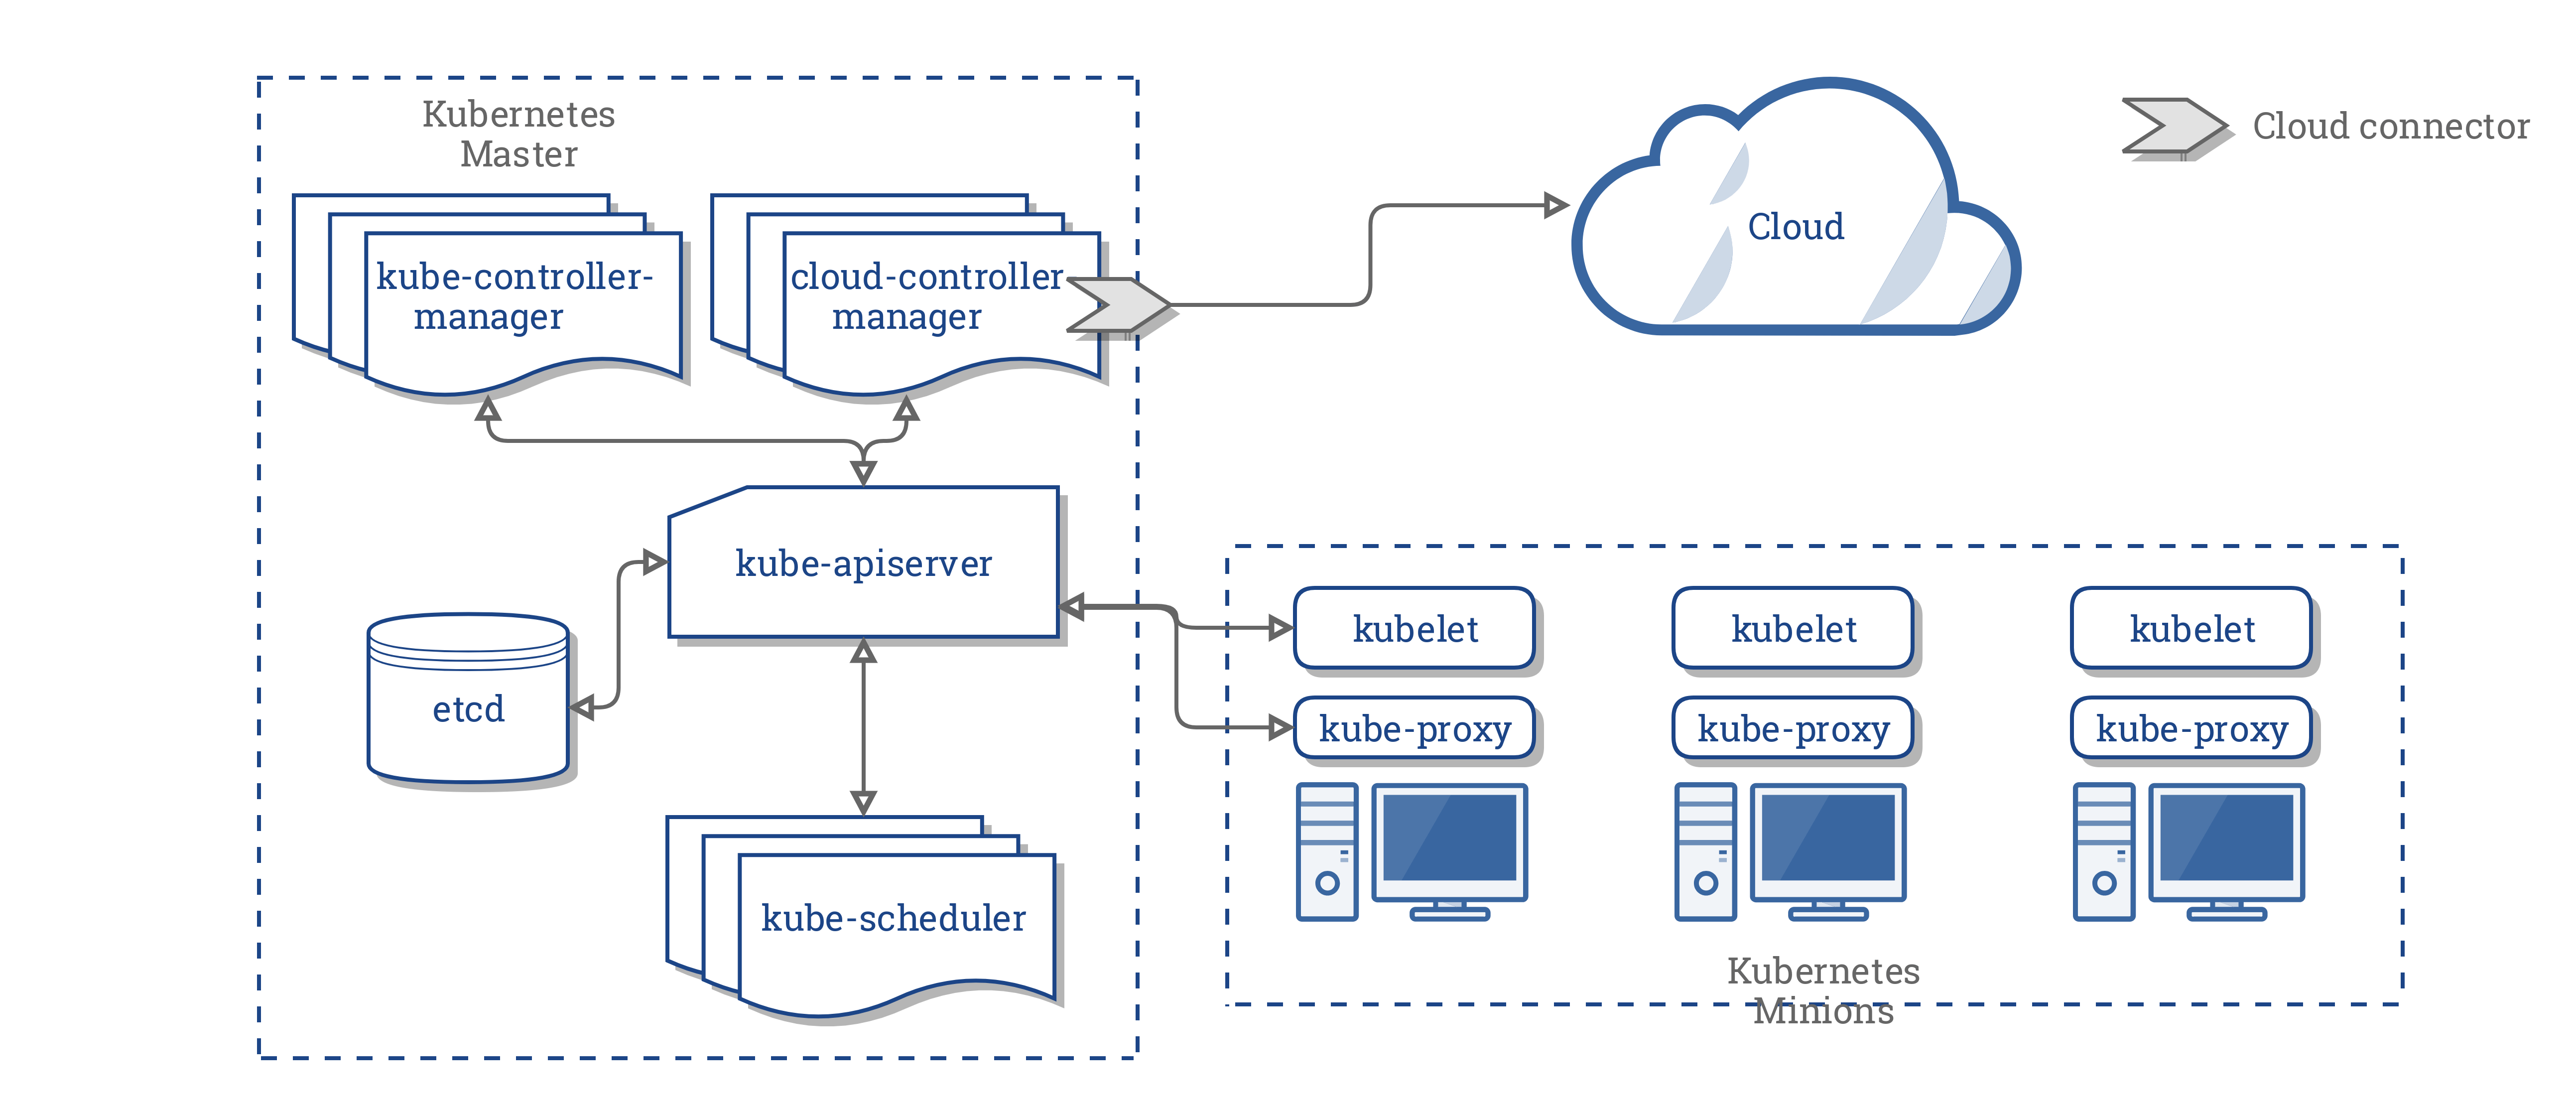
\includegraphics[width=10cm]{figures/k8s-arch.png}
	\label{fig:k8s-arch}
	\source{https://kubernetes.io/docs/concepts/architecture/cloud-controller/}
\end{figure}
\end{frame}
%}}}

\section{Available Kubernetes deployment methods}
\subsection{Using Managed Kubernetes}
\begin{frame}{Using Managed Kubernetes}%{{{
\begin{center}
	\begin{tabular}{ c c c}
		\begin{figure}
			
\includegraphics[width=3cm]{figures/managed-aws-eks.png}
			\label{fig:managed-aws-eks}
		\end{figure} &
		\begin{figure}
			
\includegraphics[width=3cm]{figures/managed-azure-kubernetes-service-aks.png}
			\label{fig:managed-azure-kubernetes-service-aks}
		\end{figure} &
		\begin{figure}
			
\includegraphics[width=4cm]{figures/managed-gcp-gke.png}
			\label{fig:managed-gcp-gke}
		\end{figure}
	\end{tabular}
\end{center}
\end{frame}
%}}}


\subsection{More custom solutions}
\begin{frame}{Using popular programs}%{{{
\begin{figure}
	
\includegraphics[width=11cm]{figures/custom-kops.png}
	\label{fig:custom-kops}
\end{figure}
\begin{figure}
	
\includegraphics[width=11cm]{figures/custom-kubeadm.png}
	\label{fig:custom-kubeadm}
\end{figure}
\begin{figure}
	
\includegraphics[width=11cm]{figures/custom-kubespray.png}
	\label{fig:custom-kubespray}
\end{figure}
\begin{figure}
	
\includegraphics[width=11cm]{figures/custom-digitalrebar-provision.png}
	\label{fig:custom-digitalrebar-provision}
\end{figure}
\end{frame}
%}}}


\subsection{Entirely customized solutions}
\begin{frame}{Entirely customized solutions}%{{{
\begin{itemize}
	\item Configuration Management frameworks: SaltStack, Ansible, Chef, Puppet
	\item Infrastructure provisioning frameworks: Terraform, CloudFormation
\end{itemize}
\end{frame}
%}}}

\section{Kubernetes cluster deployment in production environment}
\subsection{Preparations}
\begin{frame}{How to satisfy the Automation requirement?}%{{{
\textit{this is just a draft!}
\begin{itemize}
	\item TODO paste some image of a CICD pipeline
	\item TODO design 2 environments: testing and production 
\end{itemize}
\end{frame}
%}}}
\begin{frame}{How to satisfy the Security requirement?}%{{{
\textit{this is just a draft!}
\begin{itemize}
	\item HTTPS
	\item no hardcoded passwords or ssh keys
	\item maybe use a static linter 
	\item RBAC - identity and access management
\end{itemize}
\end{frame}
%}}}
\begin{frame}{How to satisfy the High Availability (HA) requirement?}%{{{
\textit{this is just a draft!}
\begin{itemize}
	\item 3 Kubernetes master nodes? etcd as a cluster
	\item at least 2 worker nodes
	\item AWS ASG (auto scaling groups)
	\item provide health checks to verify that cluster is up and running (healthy)
	\item or: blue green deployments
	\item test HA by introducing failures, measure the time needed to recover (compare with a paper)
\end{itemize}
\end{frame}
%}}}

\begin{frame}{How to satisfy the Backup and Restore requirement?}%{{{
\textit{this is just a draft!}
\begin{itemize}
	\item automated script for etcd backup 
	\item send backup outside
	\item test the restore operation
\end{itemize}
\end{frame}
%}}}

\begin{frame}{How to satisfy the Centralized Monitoring requirement?}%{{{
\textit{this is just a draft!}
\begin{itemize}
	\item use a server like Nagios, Grafana, InfluxDB, Prometheus, etc.
	\item use some AWS service e.g. CloudWatch
\end{itemize}
\end{frame}
%}}}

\begin{frame}{How to satisfy the Centralized Logging requirement?}%{{{
\textit{this is just a draft!}
\begin{itemize}
	\item use a server like Graylog, Fluentd, LogStash
	\item use some AWS service e.g. CloudWatch
\end{itemize}
\end{frame}
%}}}

\begin{frame}{How to satisfy the Centralized Audit requirement?}%{{{
\textit{this is just a draft!}
\begin{itemize}
	\item use some AWS service e.g. CloudTrail
	\item allow access to production only through CICD pipeline
\end{itemize}
\end{frame}
%}}}

\begin{frame}{How to test that k8s cluster is healthy?}%{{{
\textit{this is just a draft!}
\begin{itemize}
	\item check health status of all k8s services
	\item use a status dashboard
	\item check it every 1 minute
	\item deploy a small app on k8s to test that k8s is usable
	\item run these tests also in a CICD pipeline
\end{itemize}
\end{frame}
%}}}

\subsection{The deployment}
\begin{frame}{Method: AWS EKS}%{{{
\textit{this is just a draft!}
\begin{itemize}
	\item link to code
	\item main steps summarized
	\item overall how it went
	\item some problems + solutions 
\end{itemize}
\end{frame}
%}}}

\begin{frame}{Method: AWS with Kops}%{{{
\textit{this is just a draft!}
\begin{itemize}
	\item link to code
	\item main steps summarized
	\item overall how it went
	\item some problems + solutions 
\end{itemize}
\end{frame}
%}}}

\subsection{Comparison}
\begin{frame}{Criterium 1: Cost}%{{{
\textit{this is just a draft!}

\end{frame}
%}}}

\begin{frame}{Criterium 2: The amount of problems}%{{{
\textit{this is just a draft!}

\end{frame}
%}}}

\begin{frame}{Criterium 3: The amount of not automated resources}%{{{
\textit{this is just a draft!}

\end{frame}
%}}}

\begin{frame}{Criterium 4: Production deployment requirements met?}%{{{
\textit{this is just a draft!}

\end{frame}
%}}}

\begin{frame}{Comparison summary}%{{{
	\textit{this is just a draft!}
	\begin{tabular}{| l | c | c |}
		\hline
		& AWS EKS & AWS Kops \\
		\hline
		Cost &  &  \\
		\hline
		Problems count &  &  \\
		\hline
		Not automated resources count &  &  \\
		\hline
		Production requirements met &  &  \\
		\hline
		\end{tabular}
	\end{center}
	\end{frame}
\end{frame}
%}}}

\section{Summary}
\subsection{Lessons learned}
\begin{frame}{Lessons learned and achieved results}%{{{
	\textit{this is just a draft!}
\end{frame}
%}}}
\subsection{Future work potential}
\begin{frame}{Future work potential}%{{{
	\textit{this is just a draft!}
\begin{itemize}
	\item compare more methods of deployment
	\item use more comparison criteria - e.g. automated upgrades
	\item apply more load and run load and performance tests
	\item instead of satisfying production requirements, test enterprise and big data deployments requirements - create a survey to get lessons learned based on long running clusters and their administration
\end{itemize}
\end{frame}
%}}}
\subsection{Literature}
\begin{frame}{Literature}%{{{
	\textit{this is just a draft!}

\end{frame}
%}}}



\end{document}

